% *********************************************************************
% © 2026 Jeremy Sylvestre
%
% Permission is granted to copy, distribute and/or modify this document
% under the terms of the GNU Free Documentation License, Version 1.3 or
% any later version published by the Free Software Foundation; with no
% Invariant Sections, no Front-Cover Texts, and no Back-Cover Texts. A
% copy of the license is included in the appendix entitled “GNU Free
% Documentation License” that appears in the output document of this
% PreTeXt source code. All trademarks™ are the registered® marks of
% their respective owners.
%
% *********************************************************************
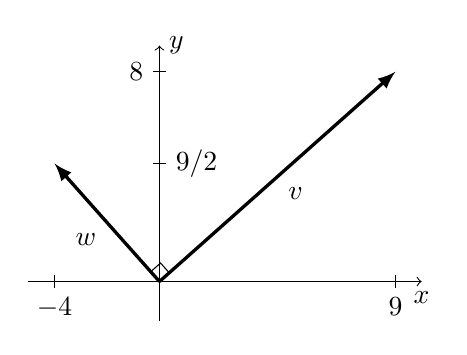
\begin{tikzpicture}[
	vector/.style={-latex,very thick},
	scale=0.333
]
	\draw[->] (-5,0) to (10,0) node[below] {$x$};
	\draw[->] (0,-1.5) to (0,9) node[right] {$y$};

	\draw[vector] (0,0) to node[below right] {$\uvec{v}$} (9,8);
	\draw[thin] (9,0.25) to (9,-0.25) node[below] {$9$};
	\draw[thin] (0.25,8) to (-0.25,8) node[left] {$8$};

	\draw[vector] (0,0) to node[below left] {$\uvec{w}$} (-4,4.5);
	\draw[thin] (-4,0.25) to (-4,-0.25) node[below] {$-4$};
	\draw[thin] (-0.25,4.5) to (0.25,4.5) node[right] {$9/2$};

	% perp symbol
	\draw[thin,rotate=41.634] (0.5,0) to (0.5,0.5) to (0,0.5);

\end{tikzpicture}
